\begin{savequote}[75mm]
Many who have had an opportunity of knowing any more about mathematics confuse it with arithmetic, and consider it an arid science. In reality, however, it is a science which requires a great amount of imagination.
\qauthor{--- Sofia Kovalevskaya ---}
\end{savequote}

\chapter{Qualitative analysis of first-order differential equations}\label{chapqualfirst}
\graphicspath{{figures/QualFirst/}}
In this chapter we will focus on a qualitative analysis of first-order differential equations that can be written as
\begin{equation}
y'=f\left(t,y\right)\,.
\label{firstorder}
\end{equation}
This means that we will not yet try to solve such equations analytically, but rather that we will resort to graphical or numerical methods to get some idea of how the solutions of the given equation behave. This is motivated because it is often impossible to find explicit formulas for solutions of differential equations. Moreover, even if there are such  formulas, they may be so complicated that they are useless. Quantitative methods of solutions for first-order differential equations will be presented in Chapter~\ref{First_Order_Quan}.

\section{Direction and vector fields}
Let us assume that Equation~\eqref{firstorder} has solutions. Recall that a solution of Equation~\eqref{firstorder} is a function $y=y(t)$ such that
$$
y'(t)=f(t,y(t))
$$
for all values of $t$ in some open interval $\left.\right]a,b\left[\right.$. Though we cannot yet solve such a differential equation analytically, we can get some insight into the shape of its solution curves by realizing that Equation~\eqref{firstorder} represents the derivative of $y(t)$ at any point $(t,y)$ in the $(t,y)$-plane, provided $f$ is continuous everywhere on this plane. This means that Equation~\eqref{firstorder} gives us a means to assess the slope of the solution curve in any point  $(t,y)$ in the $(t,y)$-plane, or put in other words, it yields the slope of the tangent line to the solution curve passing through $(t,y)$ for any  $(t,y)$ in the $(t,y)$-plane.

In practice, we evaluate the right-hand side of Equation~\eqref{firstorder} in a finite number of equidistantly spaced points $\left(t_i,y_i\right)$ in some rectangular region $R$ in the $(t,y)$-plane, and we draw short line segments of equal length through these points with slope $f\left(t_i,y_i\right)$. Moreover, we add an arrowhead to these segments pointing in the direction of increasing $t$ as we move in that direction along the solution curves with increasing $t$. The plot we obtain in this way is referred to as the \textbf{direction field} (\textit{richtingsveld}) or \textbf{slope field} of the differential equation. Since we endowed the line segments with a direction, we may as well regard them as vectors connecting the points $\left(t_i,y_i\right)$ and $\left(t_i+\Delta t,y_i+\Delta y_i\right) = \left(t_i+\Delta t,y_i+\Delta t\,f\left(t_i,y_i\right)\right)$. In that way, we do not only visualize the direction but also magnitude of the change at a given set of points. Such a plot is typically referred to as the \textbf{vector field} (\textit{vectorveld}) of a differential equation. \index{vector field}\index[aut]{vectorveld} 

Clearly, it is impracticable to construct such a direction field by hand, but fortunately this functionality is available in both Mathematica and Python. Note that the initial condition is not needed to construct the direction field. \index{direction field}\index[aut]{richtingsveld}\index{slope field}

\begin{example}
\ifmathematica
\label{exDF}
Draw the direction field of Equation~\eqref{freefall3}, i.e.
$$
m\,\dfrac{d v}{d t}=m\,g-\mu\,v\,,
$$
using Mathematica for $g=9.81$ \si{m.s^{-2}}, $m=75$ \si{kg} and $\mu=5.25$ \si{kg.s^{-1}}.

\xhrulefill{gray}{2.5pt}Solution \xhrulefill{gray}{2.5pt}

In Mathematica, this can be achieved using the function \lstinline{VectorPlot}:\index{\lstinline{VectorPlot}}\index[aut]{\lstinline{VectorPlot}}
\begin{mdframed}[default,backgroundcolor=gray!40,roundcorner=8pt]
\begin{mmaCell}[morefunctionlocal={v, t},moredefined={VectorScale,Tiny,Small}]{Input}
	 g=9.81;
	 m=75;
	 mu=5.25;
	 df=VectorPlot[\{1,g-mu*v/m\},\{t,0,30\},\{v,120,170\},VectorScale\(\pmb{\to}\)\{Tiny,Small,None\},
	
	 FrameLabel\(\pmb{\to}\)\{"Time (s)", "Velocity (m/s)"\}]

\end{mmaCell}

\begin{mmaCell}[moregraphics={moreig={scale=.4}}]{Output}
	 \mmaGraphics{FreeFall_DF.pdf}
\end{mmaCell}
\end{mdframed}
The option \lstinline{VectorScale} is used to tune the layout of the arrows in the plot. Its third argument (\lstinline{None}) dictates that the size of the line segments does not depend on the magnitude of the derivative. In other words, all plotted arrows should have the same size and we obtain the direction field. On the other hand, the vector field of the differential equation at stake can be plotted by using \lstinline{Automatic} as third argument of the option \lstinline{VectorScale} as follows

\begin{mdframed}[default,backgroundcolor=gray!40,roundcorner=8pt]
\begin{mmaCell}[morefunctionlocal={v, t},moredefined={VectorScale,Tiny,Small}]{Input}
	 g=9.81;
	 m=75;
	 mu=5.25;
	 df=VectorPlot[\{1,g-mu*v/m\},\{t,0,30\},\{v,120,170\},VectorScale\(\pmb{\to}\)\{Tiny,Small,Automatic\},
	
	 FrameLabel\(\pmb{\to}\)\{"Time (s)", "Velocity (m/s)"\}]

\end{mmaCell}

\begin{mmaCell}[moregraphics={moreig={scale=.4}}]{Output}
	 \mmaGraphics{FreeFall_VF.pdf}
\end{mmaCell}
\end{mdframed}

For completeness, let us now add the particular solution of Equation~\eqref{freefall3} satisfying $v(0)=0$ to the same plot. In Mathematica, plots can be combined using the function \lstinline{Show}:\index{\lstinline{Show}}\index[aut]{\lstinline{Show}}
\begin{mdframed}[default,backgroundcolor=gray!40,roundcorner=8pt]
\begin{mmaCell}[moredefined={ m, g, mu, VectorScale, Tiny, df}]{Input}
  v0=0;
	 sol=DSolve[\{m*D[v[t],t]==m*g-mu*v[t],v[0]==v0\},v[t],t];
	 df=VectorPlot[\{1,g-mu*\mmaFnc{v}/m\},\{\mmaFnc{t},0,30\},\{\mmaFnc{v},0,120\},VectorScale \(\pmb{\to}\)\{Tiny,Tiny,None\},
	 FrameLabel\(\pmb{\to}\)\{"Time (s)","Velocity (m/s)"\}];
	 solplot=Plot[v[\mmaFnc{t}]/.\(\pmb{\,}\)sol,\{\mmaFnc{t},0,30\},Frame\(\pmb{\to}\)True,FrameLabel\(\pmb{\to}\)\{"Time (s)","Velocity (m \mmaSup{s}{-1})"\}];
	 Show[solplot,df]
\end{mmaCell}

\begin{mmaCell}[moregraphics={moreig={scale=.7}}]{Output}
	 \mmaGraphics{FreeFall_DF2.pdf}
\end{mmaCell}
\end{mdframed}
\fi

\ifpython
\label{exDF}
Draw the direction field of Equation~\eqref{freefall3}, i.e.
$$
m\,\dfrac{d v}{d t}=m\,g-\mu\,v\,,
$$
using Python for $g=9.81$ \si{m.s^{-2}}, $m=75$ \si{kg} and $\mu=5.25$ \si{kg.s^{-1}}.

\xhrulefill{gray}{2.5pt}Solution \xhrulefill{gray}{2.5pt}

In Python, this can be achieved using the function \lstinline{quiver}:
\begin{pyin}
import numpy as np
import matplotlib.pyplot as plt
g=9.81
m=75
mu=5.25
t, v = np.meshgrid(np.linspace(0,30,15),np.linspace(120,170,14))
dt = 1
dv = g-mu*v/m

plt.quiver(t,v,dt/np.sqrt(dt**2 + dv**2),dv/np.sqrt(dt**2 + dv**2))
plt.xlabel('Time (s)')
plt.ylabel('Velocity (m/s)')
plt.show()
\end{pyin}
\begin{pyout}
|\includegraphics[width=0.5\textwidth]{FreeFall_DF_Python.png}|
\end{pyout}
The changes get divided by their scale, this dictates that the size of the line segments does not depend on the magnitude of the derivative. In other words, all plotted arrows should have the same size and we obtain the direction field. On the other hand, the vector field of the differential equation at stake can be plotted without dividing by the size

\begin{pyin}
import numpy as np
import matplotlib.pyplot as plt
g=9.81
m=75
mu=5.25
t, v = np.meshgrid(np.linspace(0,30,15),np.linspace(120,170,14))
dt = 1
dv = g-mu*v/m

plt.quiver(t,v,dt,dv)
plt.xlabel('Time (s)')
plt.ylabel('Velocity (m/s)')
plt.show()
\end{pyin}

For completeness, let us now add the particular solution of Equation~\eqref{freefall3} satisfying $v(0)=0$ to the same plot.
\begin{pyin}
import numpy as np
import matplotlib.pyplot as plt
from sympy import symbols, Function, Derivative, dsolve, lambdify
g=9.81
m=75
mu=5.25
t, v = np.meshgrid(np.linspace(0,30,15),np.linspace(0,120,14))
dt = 1
dv = g-mu*v/m
plt.quiver(t,v,dt/np.sqrt(dv**2+dt**2),dv/np.sqrt(dv**2+dt**2))

t = symbols('t')
v = Function('v')
v1 = Derivative(v(t), t)
sol = dsolve(m*v1 - m*g + mu*v(t), v(t), ics={v(0):0})
f = lambdify(t, sol.rhs, 'numpy')
t = np.linspace(0, 30, num=100)
x = np.linspace(0, 30, 100)
plt.plot(x, f(x))
plt.xlabel('Time (s)')
plt.ylabel('Velocity (m/s)')
plt.show()
\end{pyin}
\begin{pyout}
|\includegraphics[width=0.5\textwidth]{FreeFall_DF2_Python.png}|
\end{pyout}
\fi
\end{example}

From this example, it is clear that we can get a fairly accurate idea of the shape of the solution curve of a first-order differential equation given an initial condition. Essentially, it seems that we can qualitatively construct the solution curve passing through a point $(t_0,y_0)$ by following the direction indicated by the directed line segments in the direction field. This becomes even clearer if we plot the solution curves of Equation~\eqref{freefall3} for $g=9.81$ \si{m.s^{-2}}, $m=75$ \si{kg}, $\mu=5.28$ \si{kg.s^{-1}}  and an initial velocity $v_0$ varying between $0$ and $240$ \si{m.s^{-1}} on top of the direction field of the governing differential equation (Figure~\ref{FreeFallDF2}). Irrespective of the initial velocity, the direction allows us to gain qualitative insight into the shape of the solution curve. 

\begin{figure}
	\begin{center}
			\includegraphics[width=0.6\textwidth]{figures/QualFirst/FreeFall_DF3.png}
	\caption{Solutions of  Equation~\eqref{freefall3} for $g=9.81$ \si{m.s^{-2}}, $m=75$ \si{kg} , $\mu=5.28$ \si{kg.s^{-1}}  and initial velocity $v_0$ varying between $0$ and $240$ \si{m.s^{-1}} superimposed on the direction field of Equation~\eqref{freefall3}.}
	\label{FreeFallDF2}
	\end{center}
\end{figure}

The same conclusion can be drawn by inspecting an overlay of the solution curves of Equation~\eqref{eq:1.2.6}, whose interval of existence we determined in Example~\ref{example:1.2.2}, and the corresponding direction field (Figure~\ref{Example2DF}). 

\begin{figure}
	\begin{center}
			\includegraphics[width=0.6\textwidth]{Example_2_DF.pdf}
	\caption{Solution curves of Equation~\eqref{eq:1.2.6} imposed on its direction field.}
	\label{Example2DF}
	\end{center}
\end{figure}


\section{Equilibria and stability}
\label{equistab}
\subsection{Equilibrium points}
\label{equipoints}
A peculiarity about the solution curves of Equation~\eqref{freefall3} is that they seem to converge to the same constant value irrespective of the initial velocity. Besides, in Figure~\ref{FreeFallDF2} we can also see that the line segments near that value are oriented more or less horizontally, which implies locally that
$$
m\,v'=m\,g-\mu\,v\approx0\,.
$$
Clearly, there exists a velocity $v_e$ for which it holds that $v'=0$. It follows from
$$
m\,v'=m\,g-\mu\,v_e=0\,,
$$
which yields
$$
v_e=\dfrac{m\,g}{\mu}\,. 
$$
For the situation considered in Figure~\ref{FreeFallDF2}, we have $g=9.81$ \si{m.s^{-2}}, $m=75$ \si{kg} , $\mu=5.28$ \si{m.s^{-1}}, so that we find that $v_e\approx139$ \si{kg.s^{-1}}, which corresponds to the terminal velocity the solution curves in Figure~\ref{FreeFallDF2} are converging to. Once this velocity is reached, any further change of the velocity over time is impossible because $v'=0$ in $v_e$.  In general, we will refer to such points as equilibrium points.\index{equilibrium point}\index[aut]{evenwichtspunt}

\begin{definition} [Equilibrium point]
An \textbf{equilibrium point} (\textit{evenwichtspunt}) of the first-order differential equation
$$
y'=f\left(t,y\right)
$$
is any point $y_e$ for which it holds that $f\left(t,y_e\right)=0$ for all $t\geq\tau$, with $\tau$ arbitrary.
\end{definition}

This definition also indicates that $y(t)=y_e$ is a solution of the governing differential equation for all $t\geq\tau$. This solution is commonly known as an \textbf{equilibrium solution} (\textit{evenwichtsoplossing}) of the differential equation.
For an autonomous differential equation $y'=f(y)$ like Equation~\eqref{freefall3}, the equilibrium points can be retrieved easily be solving the equation $f(y_e)=0$. For most non-autonomous differential equations, however, there exist no equilibrium points. Indeed, in Figure~\ref{Example2DF} visualizing the direction field of the non-autonomous differential equation~\eqref{eq:1.2.6} no such equilibrium points can be observed. Still, there are specific non-autonomous differential equations for which one or more equilibrium points do exist.\index{equilibrium solution}\index[aut]{evenwichtsoplossing}

\subsection{Stability}
\label{1stOrderStability}

In the case of our free-falling object, it is clear that all solutions will in the end converge to the equilibrium point $v_e$ (Figure \ref{FreeFallDF2}). So, we may say that this equilibrium point attracts solutions in the neighbourhood of $v_e$, and hence acts as an \textbf{attractor} (\textit{aantrekker}). It is, however, not always that an equilibrium point attracts nearby solutions. Let us consider the following example to clarify this. \index{attractor}

\newpage

\begin{example}
\label{verhulstex}
Recall the Verhulst model we derived in Section~\ref{models} (Equation~\eqref{verhulst}), and which is based on a difference equation. Under the same assumptions, we can also derive its counterpart in continuous time. It is given by
\begin{equation}
P'=r\,P\left(1-\dfrac{P}{K}\right)\,,
\label{verhulstDE}
\end{equation}
with $P(t)$ the population size at time $t$, $r$ [T$^{-1}$] the growth rate in the absence of resource limitation, and $K$ [--] the carrying capacity of the environment. 
\index{Verhulst model}
\index[aut]{model van Verhulst}

The equilibrium points of Equation~\eqref{verhulstDE} follow from solving $P'=0$ for $P_e$
$$
r\,P_e\left(1-\dfrac{P_e}{K}\right)=0\,.
$$
Immediately, we get the two equilibrium points, namely $P_e=0$ and $P_e=K$. The obvious question now is towards which one, if any, of these two points the solution curves possibly converge for growing $t$. For that purpose, let us consider the direction field of Equation~\eqref{verhulstDE} for $K=200$ and $r=0.15$ month$^{-1}$ depicted in Figure~\ref{VerhulstDF}. Both equilibrium points can be located easily as the line segments near $P_e=0$ and $P_e=200$ are oriented almost horizontally. Suppose that we start from a strictly positive population size $N_0<K$, then we may anticipate that the solution curves will converge to the carrying capacity $K$ by studying the direction field of this differential equation. Likewise, we may anticipate that solution curves starting in points $N_0>K$ will converge to $K$. This is confirmed when we look at the general solution of Equation~\eqref{verhulstDE}, which is given by
$$
P(t)=\frac{K\,e^{C_1K+rt}}{e^{C_1K+rt}-1}\,,
$$
and whose limit for $t\to+\infty$ is $K$. 

Essentially, the fact that the solution curves converge towards $P_e=K$ does not come as a complete surprise because it is one of the equilibrium points, but $P_e=0$ is an equilibrium point as well and does not seem to attract any nearby solutions at all. Rather, it seems to be repelling them. For that reason, we will refer to a repelling equilibrium point like $P_e=0$ as an unstable equilibrium point, whereas $P_e=K$ will be referred to as an asymptotically stable equilibrium point. Besides, there exist also stable equilibrium that neither repel nor attract the solution curves. \index{unstable equilibrium point}\index[aut]{onstabiel evenwichtspunt}\index{asymptotically stable equilibrium point}\index[aut]{asymptotisch stabiel evenwichtspunt}\index{stable equilibrium point}\index[aut]{stabiel evenwichtspunt}

\begin{figure}[H]
	\begin{center}
			\includegraphics[width=0.4\textwidth]{verhulst_DF.pdf}
	\caption{Direction field of Equation~\eqref{verhulstDE} underlying the continuous-time Verhulst model.}
	\label{VerhulstDF}
	\end{center}
\end{figure}


\end{example}

Below we give more rigorous definitions of stable and asymptotically stable equilibrium points. 
\begin{definition} [Stable equilibrium point]
\label{stable}
An equilibrium point $y_e$ of the first-order differential equation
$$
y'=f\left(t,y\right)
$$
is called \textbf{stable} (\textit{stabiel}) if, given $\epsilon>0$, there is a $\delta>0$ such that $\left|y_{(t_0,y_0)}(t)-y_e\right|<\epsilon$ for all $t>0$ and for all $y_0$ such that $\left|y_0-y_e\right|<\delta$. 
\end{definition}



\begin{definition} [Asymptotically stable equilibrium point]\label{asstable}
An equilibrium point $y_e$ of the first-order differential equation
$$
y'=f\left(t,y\right)
$$
is called \textbf{asymptotically stable} (\textit{asymptotisch stabiel}) if it is stable and if $y_{(t_0,y_0)}(t)\to y_e$ as $t\to+\infty$. 
\end{definition}

An equilibrium point that is neither stable nor asymptotically stable is called \textbf{unstable} (\textit{onstabiel}). In the case of the free-falling object, it is clear that $v_e=\frac{m\,g}{\mu}$ is an asymptotically stable equilibrium point as the directed line segments in the corresponding direction field (Figure~\ref{FreeFallDF2}) point towards this velocity. 

Stability of an equilibrium point can be illustrated as well intuitively by imagining a ball at rest on a hill or in a valley (Figure~\ref{ballStability}). When the ball is at rest on top of a hill, the slightest push will cause the ball to roll away (Figure~\ref{Instabiel}), which represents the behaviour of solutions near an unstable equilibrium point. Conversely, a ball in a valley will, when pushed, return to its resting position (Figure~\ref{Stabiel}).

\begin{figure}[H]
\centering
%\raisebox{0.5cm}{
\centerline{
\subfigure[\label{Instabiel}]{\includegraphics[width=0.3\textwidth]{figures/QualFirst/Instabiel.pdf}}
\hspace{1cm}
\subfigure[\label{Stabiel}]{\includegraphics[width=0.3\textwidth]{figures/QualFirst/Stabiel.pdf}}
}
\caption{Visual representation of an unstable (a) and stable (b) equilibrium.}\label{ballStability} 

\end{figure}


Recall that the right-hand side $f\left(t^*,y^*\right)$ of a differential equation in a point $(t^*,y^*)$ tells us whether the solution curve described by $y(t)$ and passing through $(t^*,y^*)$ is increasing ($f\left(t^*,y^*\right)>0$) or decreasing ($f\left(t^*,y^*\right)<0$) in that point. In the case of an autonomous differential equation $y'=f(y)$, this is even completely determined by $y^*$ only because $t$ does not appear explicitly in its right-hand side. Hence, given $y^*$ one can verify whether the solution through that point will evolve towards values greater or smaller than $y^*$, and consequently whether the solution curve will converge to some equilibrium point, remains close to it, or is repelled by it. So, by studying the graph of $f(y)$ it should be possible to infer the stability of the possible equilibrium points of $y'=f(y)$. For the sake of clarity, we adopt the convention that asymptotically stable equilibrium points on such graphs are marked with filled circles and unstable equilibrium points with open circles.

\begin{example}
Consider the graphs of the functions corresponding to the right-hand sides of Equations~\eqref{freefall3} and \eqref{verhulstDE} in Figure~\ref{Y_Ydot_Free_Fall} and~\ref{Y_Ydot_Verhulst}, respectively. In these figures the red arrows indicate the direction to which solutions evolve over time.

From the former we may conclude that $v'$ is positive for all velocities $v<v_e$, while it is negative for all $v>v_e$. This implies that $v_{(t_0,v_0)}(t)$ increases monotonically up to the point where the solution curve reaches the terminal velocity $v_e$ for all $v_0<v_e$, whereas the opposite is true if $v_0>v_e$. Essentially, this corresponds to our physical understanding of this process: a free-falling object will accelerate up to a certain terminal velocity when starting its fall with an initial velocity that was lower than the terminal one, whereas it will decelerate when it started its fall at $v_0>v_e$.  Once the terminal velocity is reached, there is an equilibrium between the gravitational and frictional forces. 

A similar reasoning allows us to understand that $P_e=K$ is an asymptotically stable equilibrium point of Equation~\eqref{verhulstDE}, whereas $P_e=0$ is an unstable equilibrium point. Indeed, $P'>0$ for all $P<K$, so the population size will gradually increase when it was initially lower than the carrying capacity  $K$, and vice versa when the population was initially greater than the carrying capacity $K$. Again, this corresponds to our intuition of the process. Note by the way that the function $f(P)$ is decreasing in $P_e=K$, whereas it is increasing in $P_e=0$. This intuitive insight into the link between the stability of an equilibrium point and the derivative of the right-hand side of the differential equation at the equilibrium point is formalized in Theorem~\ref{firstdifftest}. 

\begin{figure}[H]
\centering
%\raisebox{0.5cm}{
\centerline{
\subfigure[\label{Y_Ydot_Free_Fall}]{\includegraphics[width=0.49\textwidth]{Y_Ydot_Free_Fall}}
\hspace{0.1cm}
\subfigure[\label{Y_Ydot_Verhulst}]{\includegraphics[width=0.49\textwidth]{Y_Ydot_Verhulst}}
}
\caption{Graphs of the functions corresponding to the right-hand sides of Equations~\eqref{freefall3} (a) and \eqref{verhulstDE} (b), with their asymptotically stable and unstable equilibrium points (filled and open circles, respectively) and the direction to which the solutions evolve over time (red arrows).} 

\end{figure}
\end{example}

\newpage 
\begin{theorem}[First derivative test]
\label{firstdifftest}
Suppose that $y_e$ is an equilibrium point of the autonomous differential equation
$$
y'=f\left(y\right)\,,
$$
where $f$ is a differentiable function. 
\begin{enumerate}
	\item If $f'\left(y_e\right)<0$, then $y_e$ is asymptotically stable.
	\item If $f'\left(y_e\right)>0$, then $y_e$ is unstable.
	\item If $f'\left(y_e\right)=0$, then no conclusion can be drawn solely on the basis of $f'\left(y_e\right)$.
\end{enumerate}
\end{theorem}
\index{first derivative test}
\index[aut]{eerste-afgeleide test}

Using this theorem one can in most cases easily determine the stability of the equilibrium point of an autonomous differential equation. Yet, if $f'\left(y_e\right)=0$ different situations are possible, one of which is illustrated in Figure~\ref{First_Diff_Test0}. Since $y'=0$ for all $y$ in the interval $[2,4]$, there are infinitely many equilibrium points, namely $[2,4]$. For all of them, it holds that $f'\left(y_e\right)=0$, so Theorem~\ref{firstdifftest} is of no help to determine their stability. Yet, since $y'$ is positive for all $y<2$, it is obvious that for any $y_0<2$ we will have $y_{(t_0,y_0)}(t)$ converges to 2. Likewise, for any $y_0>4$ we will have $y_{(t_0,y_0)}(t)$ converges to 4. On the other hand, solution curves originating from a point $y_0$ lying in $[2,4]$ will stay at that point, and will not be attracted by other points. Hence, these solutions will be given by $y(t)=y_0$ because $y'=0$ in any of these points. Consequently, in the light of Definition~\ref{stable}, the infinitely many equilibrium points in $[2,4]$ are stable. Sometimes the points at the boundaries of the interval $[2,4]$, i.e.\ $y_e=2$ and $y_e=4$, are referred to as \textbf{semi-asymptotically stable equilibrium points} (\textit{semi-asymptotisch evenwichtspunt}) because solution curves originating from points to left of the former converge to $y_e=2$, whereas there is no such convergence for solution curves originating from $y_0$ in $[2,4]$, and likewise for $y_e=4$. Moreover, in cases where solutions on one side of an equilibrium point move towards the equilibrium point and on the other side of the equilibrium point move away from it, we call the equilibrium point \textbf{semi-stable} (\textit{semi-stabiel}). Such equilibrium points will be indicated by means of triangular markers. 
\index{semi-stable equilibrium}
\index[aut]{semi-stabiel evenwichtspunt}
\index{semi-asymptotically stable equilibrium}
\index[aut]{semi-asymptotisch stabiel evenwichtspunt}

\begin{figure}[H]
	\begin{center}
			\includegraphics[width=0.5\textwidth]{First_Diff_Test0.pdf}
	\caption{Graph of $f(y)$ for an autonomous differential equation $y'=f\left(y\right)\,$, with $f'\left(y_e\right)=0$.}
	\label{First_Diff_Test0}
	\end{center}
\end{figure}

\newpage

\begin{example}
Determine the equilibrium points of the following differential equation
\begin{equation}
y'=y^3-2\,y^2-y+2\,,
\label{vbfirstdifftest}
\end{equation}
as well as their stability. 

\xhrulefill{gray}{2.5pt}Solution \xhrulefill{gray}{2.5pt}

The equilibrium points of Equation~\eqref{vbfirstdifftest} follow from:
\begin{eqnarray*}
0&=&y_e^3-2\,y_e^2-y_e+2\,,\\
&=&\left(y_e^2-1\right)\left(y_e-2\right)\,.
\end{eqnarray*}
So, the equilibrium points of Equation~\eqref{vbfirstdifftest} are $y_e=-1$, $y_e=1$ and $y_e=2$. To determine their stability, we consider the first-order derivative of the right-hand side of Equation~\eqref{vbfirstdifftest} with respect to $y$:
$$
y''=f'(y)=3\,y^2-4\,y-1\,.
$$
Evaluating $f'(y)$ in each of the equilibrium points, yields $f'(-1)=6$, $f'(1)=-2$ and $f'(2)=3$, so by relying on Theorem~\ref{firstdifftest}, we may conclude that both $y_e=-1$ and $y_e=2$ are unstable equilibrium points, whereas $y_e=1$ is an asymptotically stable equilibrium point. This is confirmed by Figure~\ref{vbfigfirstdifftest} that shows both the graph of $f(y)$ and the direction field of Equation~\eqref{vbfirstdifftest}.

\begin{figure}[H]
\centering
%\raisebox{0.5cm}{
\centerline{
\subfigure[]{\includegraphics[width=0.55\textwidth]{vbfirstdifftest1}}
\hspace{0.1cm}
\subfigure[]{\includegraphics[width=0.35\textwidth]{vbfirstdifftest2}}
}
\caption{Graph of the right-hand side (a) and direction field (b) of Equation~\eqref{vbfirstdifftest}. On the former the asymptotically stable equilibrium points are marked with filled circles and unstable equilibrium points with open circles. The direction to which the solutions evolve over time is indicated by red arrows. } 
\label{vbfigfirstdifftest}
\end{figure}

\end{example}


\section{Bifurcation}
In Example~\ref{verhulstex} we already observed that the value of an equilibrium point might depend on a model parameter; that is the carrying capacity $K$ in the case of the Verhulst model.  Moreover, we encountered an example where the specific value depends even on more than one parameter. Indeed, the equilibrium velocity of a free-falling object that is subject to gravitational and frictional forces is given by $v_e=\frac{m\,g}{\mu}$, which depends on three parameters. 

Not only can model parameters affect the value of an equilibrium point, they might as well have a decisive impact on its stability and even affect the number of equilibrium points. For instance, it might happen than for a certain range of parameter values an equilibrium point $y_e$ is asymptotically stable, whilst it is unstable for parameter values outside this range, or vice versa. This phenomenon is known as \textbf{bifurcation} (\textit{bifurcatie}) and plays an important role in the analysis of many mathematical models. A parameter $p$ that gives rise to bifurcation is referred to as a \textbf{bifurcation parameter} (\textit{bifurcatieparameter}). The effect of a bifurcation parameter on the stability and/or number of equilibrium points is typically summarized in a so-called \textbf{bifurcation diagram} (\textit{bifurcatiediagram}), which visualizes the equilibrium points and their stability as a function the bifurcation parameter $p$. For what concerns the bifurcation diagram, we adopt the convention that asymptotically equilibrium points will be indicated by means of a solid line, while a dashed line will be used to indicate unstable equilibrium points. \index{bifurcation}\index[aut]{bifurcatie}\index{bifurcation parameter}\index[aut]{bifurcatieparameter}\index{bifurcation diagram}\index[aut]{bifurcatiediagram}

\begin{definition} [Bifurcation point]
A \textbf{bifurcation point} (\textit{bifurcatiepunt}) of the autonomous differential equation
$$
y'=f_p\left(y\right)\,,
$$
where $p$ is a real bifurcation parameter, is the parameter value $p^*$ where there is a change in the number and/or stability of equilibrium points. 
\end{definition}

Depending on the transition that happens when crossing from one side of a bifurcation point to the other side along the parameter axis, we distinguish three main types of bifurcation when there is one parameter, which are illustrated in Figure~\ref{bifurcaties}. 
\begin{itemize}
	\item \textbf{Saddle-node bifurcation} (\textit{zadel-knoop bifurcatie}): this manifests itself when there is one equilibrium point in the bifurcation point $p^*$, two at one side of $p^*$ and none at the other side (Figure~\ref{saddle}). 
	\item \textbf{Transcritical bifurcation} (\textit{transkritische bifurcatie}): this happens when there are always two equilibrium points, irrespective of the value of the bifurcation parameter, but these points exchange their stability when we move across the bifurcation point $p^*$ (Figure~\ref{transcritical}).
	\item \textbf{Pitchfork bifurcation} (\textit{hooivorkbifurcatie}): this kind of bifurcation can be observed when there is one equilibrium point at one side of the bifurcation point $p^*$, while there are three at the other side (Figure~\ref{pitchfork}). 
\end{itemize}
\index{saddle-node bifurcation}\index[aut]{zadel-knoop bifurcatie}\index{pitchfork bifurcation}\index[aut]{hooivorkbifurcatie}\index{transcritical bifurcation}\index[aut]{transkritische bifurcatie}

\begin{figure}[h]

\centerline{
\subfigure[\label{saddle}]{\includegraphics[width=0.31\textwidth]{saddle}}
\hspace{0.1cm}
\subfigure[\label{transcritical}]{\includegraphics[width=0.31\textwidth]{transcritical}}
\hspace{0.1cm}
\subfigure[\label{pitchfork}]{\includegraphics[width=0.31\textwidth]{pitchfork}}
}
%\centerline{
%\subfigure[\label{pitchfork}]{\includegraphics[width=0.31\textwidth]{pitchfork}}
%}
\caption{Possible bifurcations: saddle-node (a), transcritical (b) and pitchfork (c). The bifurcation point is indicated by means of a square marker.} 
\label{bifurcaties}
\end{figure}

\newpage

\begin{example}
Consider the autonomous differential equation
\begin{equation}
y'=p+y^2\,,
\label{vbbifurcatie}
\end{equation}
where $p$ is a real parameter. Determine the equilibrium point(s) of this differential equation and its (their) stability as a function of the parameter $p$. 

\xhrulefill{gray}{2.5pt}Solution \xhrulefill{gray}{2.5pt}

The equilibrium point(s) of Equation~\eqref{vbbifurcatie} is (are) given by
$$
y_e=\pm\sqrt{-p}\,.
$$
From this we already infer that there are two equilibrium points if $p<0$, none if $p$ is positive and one if $p=0$, so $p=0$ is the bifurcation point, and we are faced with a saddle-node bifurcation. Figure~\ref{vbbifurcatiefig} shows a typical plot of the right-side of Equation~\eqref{vbbifurcatie} for each of the three parameter settings. From Figure~\ref{vbbifurcatiefigneg}, we may conclude that for $p<0$ the equilibrium points $y_e=+\sqrt{-p}$ are unstable, while the equilibrium points $y_e=-\sqrt{-p}$ are asymptotically stable. Figure~\ref{vbbifurcatiefigpos} confirms that there are no equilibrium points if $p>0$, while Figure~\ref{vbbifurcatiefig0} demonstrates that $y_e=0$ is a semi-stable equilibrium point if $p=0$. All this information is summarized in the bifurcation diagram depicted in Figure~\ref{vbbifurcatiediag}.\index{saddle-node bifurcation}\index[aut]{zadel-knoop bifurcatie}

\begin{figure}[H]

\centerline{
\subfigure[$p = -1$\label{vbbifurcatiefigneg}]{\includegraphics[width=0.31\textwidth]{vbbifurcatiefigneg}}
\hspace{0.1cm}
\subfigure[$p = 1$\label{vbbifurcatiefigpos}]{\includegraphics[width=0.31\textwidth]{vbbifurcatiefigpos}}
\hspace{0.1cm}
\subfigure[$p = 0$\label{vbbifurcatiefig0}]{\includegraphics[width=0.31\textwidth]{vbbifurcatiefig0}}
}
%\centerline{
%\subfigure[$p = 0$\label{vbbifurcatiefig0}]{\includegraphics[width=0.49\textwidth]{vbbifurcatiefig0}}
%}
\caption{Plots of the right-hand side of Equation~\eqref{vbbifurcatie} for $p<0$ (a), $p>0$ (b) and $p=0$ (c).} 
\label{vbbifurcatiefig}
\end{figure}

\begin{figure}[H]
	\begin{center}
			\includegraphics[width=0.6\textwidth]{vbbifurcatiediag}
	\caption{Bifurcation diagram of Equation~\eqref{vbbifurcatie}.}
	\label{vbbifurcatiediag}
	\end{center}
\end{figure}
\end{example}

To conclude, let us investigate whether bifurcation plays a role in a modified version of the Verhulst model that accounts for harvesting of the population.

\begin{example}
\label{exbifverhulst}
We can easily extend Equation~\eqref{verhulstDE} to account for the harvesting of individuals at a certain rate $h$ [T$^{-1}$], assuming that the harvested number of individuals is proportional to the number of individuals in the population, i.e.
\begin{equation}
	P'=r\,P\left(1-\dfrac{P}{K}\right)-h\,P\,.
\label{verhulstDE2}
\end{equation}
The equilibrium points of Equation~\eqref{verhulstDE2} follow from solving
$$
0=r\,P_e\left(1-\dfrac{P_e}{K}\right)-h\,P_e
$$
for $P_e$, which yields $P_e=0$ and $P_e=K\left(1-\frac{h}{r}\right)$. As in Example~\ref{verhulstex}, let us assume that $K=200$ and $r=0.15$ month$^{-1}$, so that the latter equilibrium point becomes 
$$
P_e=200\left(1-\frac{h}{0.15}\right)\,.
$$
Consequently, there are two equilibrium points irrespective of the harvest rate $h$. In order to verify whether the harvest rate $h$ can affect the stability of these equilibrium, we compute the derivative of the right-hand side of Equation~\eqref{verhulstDE2} with respect to $P$, which yields
$$
f'(P)=r-\frac{2\,r\,P}{K}-h=\frac{3}{20}-\frac{3\,P}{2000}-h\,,
$$
so that we can apply the first-derivative test (Theorem~\ref{firstdifftest}) at both equilibrium points. At $P_e=0$ we get $f'(0)=0.15-h$, whereas we obtain 
$$
f'\left(200\left(1-\frac{h}{0.15}\right)\right)=h-0.15\,.
$$
It is clear that the sign of these expressions depends on the harvest rate $h$. More precisely, we see that $P_e=0$ is asymptotically stable for all $h>0.15$, whereas it is unstable for $h<0.15$, and the first-derivative test is inconclusive for $h=0.15$. Likewise, we see that $P_e=200\left(1-\frac{h}{0.15}\right)$ is asymptotically stable for all $h<0.15$, whereas it is unstable for $h>0.15$, and the first-derivative test is inconclusive for $h=0.15$. We may conclude that Equation~\eqref{verhulstDE2} has a bifurcation point at $h=0.15$, where the equilibrium points exchange their stability. Consequently, Equation~\eqref{verhulstDE2} gives rise to a transcritical bifurcation. Figure~\ref{bifurcatiediagcverhulst} shows the corresponding bifurcation diagram. It is obvious that $P_e=0$ is the only ecologically relevant equilibrium point if $h>0.15$.\index{transcritical bifurcation}\index[aut]{transkritische bifurcatie}

\begin{figure}[H]
	\begin{center}
			\includegraphics[width=0.6\textwidth]{bifurcatiediagcverhulst}
	\caption{Bifurcation diagram of Equation~\eqref{verhulstDE2}.}
	\label{bifurcatiediagcverhulst}
	\end{center}
\end{figure}


\end{example}


The outcome of the analysis in Example~\ref{exbifverhulst} also corresponds with our ecological intuition: if individuals are harvested faster than they can reproduce the populations must go extinct in the long run. It is argued that such a tipping point might exist in many ecosystems, in the sense that its recovery becomes impossible if the disturbance rate/frequency exceeds a certain threshold. For that reason, it is important to be able to study the governing models from a qualitative point of view because one gets insight into the possible equilibrium states of ecosystems and the drivers that might bring it to a collapse. 


\newpage
\section{Exercises} % Alles komt uit de bordoefeningen of practica van W3. Nog te herwerken naar Python.
%\subsection{General}
\subsection{Direction and vector fields}

Direction fields can also be plotted in Python. For this purpose the function \texttt{directionfield} is available in the script \texttt{directionfield.py}, the implementation of which is given below:
\begin{lstlisting}
def richtingsveld(f, tinterval, yinterval, n = 25):  
    tmin = tinterval[0]
    tmax = tinterval[1]
    ymin = yinterval[0]
    ymax = yinterval[1]
    T = numpy.linspace(tmin, tmax, n)
    y = numpy.linspace(ymin, ymax, n)
    #Vector field
    [X, Y] = numpy.meshgrid(T, y)
    U = 1
    V = f(T, Y)
    #Normalize arrows
    N = numpy.sqrt(U**2 + V**2)  
    U = U/N
    V = V/N
    plt.quiver(X, Y, U, V)    
    plt.xlim(tinterval)
    plt.ylim(yinterval)
    plt.xlabel('$t$')
    plt.ylabel('$y$')
    plt.show()
\end{lstlisting}


The function \texttt{directionfield} has the following inputs:
\begin{enumerate}
	\item \texttt{f}:the right-hand side of the differential equation,
	\item \texttt{tinterval}: the considered time interval,
	\item \texttt{yinterval}: the considered $y$ interval, and
	\item \texttt{n}: precision of the direction field, default is $n = 25$.
\end{enumerate}
To illustrate, consider the following differential equation describing the dynamics of a population of size $P$:

\begin{equation}\label{verhulstDE3}
P' = r\,P\left(1-\dfrac{P}{K}\right) - h\,P\,, \qquad P(0) = 5\,,
\end{equation}

with $h$ [T$^{-1}$] the rate at which the population is harvested (cf.\ Equation~\eqref{verhulstDE2} from Example~\ref{exbifverhulst}). We first implement the right-hand side in Python as the function \texttt{exampleRL} with $r = 1.5$, $K = 2$, and $h = 1$ s$^{-1}$:
\begin{lstlisting}
def voorbeeldRL(t, P):
    r = 1.5
    K = 2
    h = 1
    ydot = r*P*(1 - P/K) - h*P
    return ydot
\end{lstlisting}

Note that, although the right-hand side does not explicitly depend on $t$, it is always given as the first input.

The corresponding direction field can now be easily plotted by entering the following instruction in the instruction window:
\begin{lstlisting}
richtingsveld(voorbeeldRL, [0, 10], [0, 5], 25)
\end{lstlisting}

The result is shown in Figure~\ref{fig:voorbeeldRV}.

\begin{figure}[ht]
\centering
\includegraphics[width=8cm]{richtingsveldVB.png}\\
\caption{The direction field of Equation\ \eqref{verhulstDE3} with $r = 1.5$, $K = 2$, and $h = 1$.\label{fig:voorbeeldRV}}
\end{figure}

\begin{Exercise} Consider the first-order differential equation
\begin{equation}\label{EqK1}
y' = y\,\left(-2\,t + \frac{1}{t}\right)\,
\end{equation}
over the $t$-interval $[0.2,\, 3]$, with initial condition $y\left(0.2\right)=0.2$.
\ifmathematica

    \Question Determine the exact solution of differential equation \eqref{EqK1} using Mathematica. % $y(t)=t\,e^{0.04-t^2}$
    \Question Plot the direction field of differential equation \eqref{EqK1} over the time interval $[0.2,3]$ and the $y$-interval $[0,1]$. First, implement the right-hand side in Python. To do this, complete the script \textit{function1.py}:
\begin{lstlisting}[caption=functie1]
def functie1(t, y):
    ydot = 
    return ydot
\end{lstlisting}
    \Question Plot on top of the obtained direction field the exact solution you obtained with Mathematica.
\fi

\ifpython
    \Question Determine the exact solution of differential equation \eqref{EqK1} using Python. % $y(t)=t\,e^{0.04-t^2}$
    \Question Plot the direction field of differential equation \eqref{EqK1} over the time interval $[0.2,3]$ and the $y$-interval $[0,1]$.First, implement the right-hand side in Python. To do this, complete the script \texttt{function1.py}:
\begin{lstlisting}[caption=functie1]
def functie1(t, y):
    ydot = 
    return ydot
\end{lstlisting}
    \Question Plot on top of the obtained direction field the exact solution you obtained with Python.
\fi
\end{Exercise}

\setboolean{firstanswerofthechapter}{true}
\begin{Answer}\phantom{}
    	\Question The exact solution we find with \ifmathematica Mathematica \fi \ifpython Python \fi is $y(t) = 1.04081e^{-t^2}t$. If however you use 1/5 instead of 0.2, you get: $y(t) = e^{1/25 - t^2}t$.
    	\Question The directional field of the given differential equation can be seen in \ref{fig:oefening2_1}
    	\Question With the instructions below we get Figure~ \ref{fig:oefening2_1}.

\begin{lstlisting}
direction field(function1, [0.2, 3], [0, 1], 25)
t = arange(0.2, 3, 0.1)
y = t*exp(1/25 - t**2)
plt.plot(t, y, 'r.')
\end{lstlisting}
        
\begin{figure}[H]
	\centering				\includegraphics[width=10cm]{oefening2_1.png}\\
	\caption{Direction field and exact solution of $y' = y(-2t + 1/t)$. \label{fig:oefening2_1}}
\end{figure}
    
    \EndCurrentQuestion
\end{Answer}
\setboolean{firstanswerofthechapter}{false}

\begin{Exercise} Consider the following first-order differential equation over the $t$ interval $[-2,\,2]$:
$$y'=y+3\,t-t^3.$$

\Question Implement the right-hand side of this differential equation in Python as \texttt{function2} in the script \texttt{function2.py}.
\Question Plot the direction field of this differential equation. Set the $y$-axis to $[-2,\,2]$.
\Question Describe what happens when you increase the precision $n$. For example, set $n$ equal to 10, 20, 50, and 100.
\Question Can you predict the global course of the exact solution through the point $(-2,0.5)$ using this plot?
\ifmathematica
\Question Determine the general solution of this differential equation using Mathematica.
\fi
\ifpython
\Question Determine the general solution of this differential equation using Python.
\fi
\ifmathematica
\Question Use Mathematica to determine the exact solution of the differential equation through the point $(-2,0.5)$ and implement this solution in Python as \texttt{exact2}. Optionally use \texttt{Simplify} to simplify the obtained solution. Plot the exact solution through $(-2,0.5)$ on top of the direction field. Does the result match the trend predicted in (d)?
\fi
\ifpython
\Question Use Python to determine the exact solution of the differential equation through the point $(-2,0.5)$ and implement this solution in Python as \texttt{exact2}. Optionally use \texttt{Simplify} to simplify the obtained solution. Plot the exact solution through $(-2,0.5)$ on top of the direction field. Does the result match the trend predicted in (d)?
\fi
%\ifmathematica
%\item Use Mathematica to determine the unique solution of the differential equation for the generic initial values $y(t_0)~=~y_0$.
%\fi
%\ifpython
%\item  Use Python to determine the unique solution of the differential equation for the generic initial values $y(t_0)~=~y_0$.
%\fi
%$$
%y \left( t \right) =3+3\,t+3\,{t}^{2}+{t}^{3}-{\frac {{e^{t}} \left( -
%{\it y0}+3+3\,{\it t0}+3\,{{\it t0}}^{2}+{{\it t0}}^{3} \right) }{{e^{
%{\it t0}}}}}.$$
%\itemVisualize the exact solutions at different initial conditions on top of the direction field if $t_0=-2$ and $y_0 \in \left\{0,\tfrac{1}{4}, \tfrac{1}{2}, \tfrac{3}{4}, 1, \tfrac{5}{4}, \tfrac{3}{2}\right\}$. Use the following script for this:

%\begin{lstlisting}[caption=ploty0]
%fplot(@(t)exact1t0(t, -2, 0:0.25:1.5), [-2, 2])
%\end{lstlisting}

%Discuss what you see.
\end{Exercise}

\begin{Answer}\phantom{}
    	\Question /
    	\Question The direction field of the given differential equation can be seen in \ref{fig:oefening2_2}.
        \Question When the precision $n$ increases, more direction vectors are shown in the direction field.
        \Question You can predict the global course of the exact solution by following the direction vectors from the point $(-2,0.5)$.
        \Question The general solution we determine with Mathematica, is $y(t) = 3+3t+3t^2+t^3+e^tC[1]$
        \Question The exact solution through the point $(-2,0.5)$ is (after simplification with \texttt{Simplify}) \\ $y(t) = 3 - \dfrac{e^{2+t}}{2} + 3t + 3t^2 + t^3$. After implementation in Python as \texttt{exact2} and plotting on top of the directional field, you get Figure \ref{fig:oefening2_2}.

\begin{figure}[H]
	\centering				\includegraphics[width=10cm]{oefening2_2.png}\\
	\caption{Direction field and exact solution of $y' = y + 3t - t^3$.}
	\label{fig:oefening2_2}
\end{figure}

    \EndCurrentQuestion
\end{Answer}

%\item During the night of January 3, an unknown person discharged a few barrels of a toxic substance into the the Coupure. One day after the incident, samples are taken near the discharge site. The analysis shows that the concentration of the toxic substance on that day was \num{1.25e-2} \si{\mole.\meter^{-3}}. Students from the Faculty of Bioscience Engineering used a differential equation to predict the concentration of the toxic substance over time. Figure \ref{figH24} illustrates the direction field that this model yielded. Will the toxic substance still be detectable after 50 days if the detection limit is \num{5e-3}\si{\mole.\meter^{-3}}?\vspace*{1cm}
%\begin{figure}[h]
%\centering
%%\raisebox{0.5cm}{
%\includegraphics[width=12cm]{figH24.eps}%}
%\caption{Direction field for predicting the concentration of toxic substance as a function of time.} \label{figH24}
%\end{figure}



\begin{Exercise}\label{oef2} Consider the four direction fields depicted in Figure~\ref{figH26}. 
\begin{figure}[h!]
\centerline{
\subfigure[Richtingsveld I]{\includegraphics[width=8cm]{figH25.eps}
\label{Fig1a}}
\hfil
\subfigure[Richtingveld II]{\includegraphics[width=8cm]{figH26.eps}
\label{Fig1b}}}
\centerline{
\subfigure[Richtingsveld III]{\includegraphics[width=8cm]{figH27.eps}
\label{Fig1c}}
\hfil
\subfigure[Richtingsveld IV]{\includegraphics[width=8cm]{figH28.eps}
\label{Fig1d}}}
\caption{Direction fields from Exercise \ref{oef2}. \label{figH26}}
\end{figure}

Which differential equation corresponds to which direction field? Justify your answer.

\begin{multicols}{2}
\begin{enumerate}
\item $y' =\sin\left(y\right)$
\item $y'= \displaystyle\frac{y}{t}$
\item $y'= \displaystyle\frac{t}{y}$
\item $y'= t+y$
\end{enumerate}
\end{multicols}
\EndCurrentQuestion
\end{Exercise}

\begin{Answer}
        \begin{multicols}{2}
        \Question III
        \Question I
        \Question II
        \Question IV
        \EndCurrentQuestion
        \end{multicols}
\end{Answer}
%\item Consider the DE
%$$
%y'= y^4+2\, y^3-3\, y^2-8\, y -4\,,
%$$ 
%of which the right-hand side is depicted in Figure~\ref{fig:evenwicht2}.

%\begin{enumerate}
%\item Find and classify the equilibrium points in $\left[-2.5,2.5\right]$ of this DE.
%\item Also indicate the direction of movement of an object located in the point $a$, $b$ or $c$  on the horizontal axis.%\vspace{1.2cm}
%\item If we limit the $y$ interval over which we consider the DE to $[-1, 2.5[$, does this change the number of equilibrium points and their stability? \vspace*{1.5cm}
%\begin{figure}[h!]
%\centering
%\raisebox{0.5cm}{
%\includegraphics[width=12cm]{figH23.eps}%}
%\caption{Plot of the DE  $y'= y^4+2\, y^3-3\, y^2-8\, y -4$.} \label{fig:evenwicht2}
%\end{figure}
%\end{enumerate}

%\item Consider the following first-order DEs, where $p$ represents a real parameter.
%\begin{enumerate}
%    \item $y'=p\,y-y^3$
%    \item $y'=y^2+4\,p^2-1$
%\end{enumerate}
% Determine the equilibrium point(s) of these DEs as a function of the real parameter $p$. Then sketch the bifurcation diagram and indicate the stability of the equilibrium points on it.





\pagebreak
\subsection{Equilibria and stability}
\begin{Exercise} Determine analytically the equilibrium points of the following differential equations. Check your results with \ifmathematica Mathematica. \fi  \ifpython Python. \fi
				\Question $y' = (y - 4)(y + 1)$
				\Question $y' = y^2(6 - y)$
				\Question $y' = y^2 - y - 6$
				\Question $y' = y^3 - 4y$
				\Question $y'=2\,\sqrt y$
				\Question $N' = r\,N\left(1 - \dfrac{N}{K}\right) - p\,N$ \quad with $r = 2.5$, $K = 250$, and $p = 0.2$
                \Question $y'=h(t-1)$,\quad where $h(t)=1$ if $t\geq0$ and $h(t)=0$ else
    \EndCurrentQuestion
\end{Exercise}

\begin{Answer}
    \begin{multicols}{2}
        \Question $y_e = -1$ \quad and \quad $y_e = 4$
        \Question $y_e = 0$ \quad and \quad $y_e = 6$
        \Question $y_e = -2$ \quad and \quad $y_e = 3$
        \Question $y_e = 0$ \quad and \quad $y_e = \pm2$
        \Question $y_e = 0$
        \Question $N_e = 0$ \quad and \quad $N_e = (p-r)\dfrac{K}{r}$
        \Question no equilibrium points
        \EndCurrentQuestion
    \end{multicols}
    
    Checking the results for the third differentail equation:
        \begin{mdframed}[default,backgroundcolor=gray!40,roundcorner=8pt]
        \begin{mmaCell}{Input}
          Solve[\{0 == y^2 - y - 6 \}, y]
        \end{mmaCell}

        \begin{mmaCell}{Output}
        	 \{\{y \(\to\) -2\}, \{y \(\to\) 3\}\}
        \end{mmaCell}
        \end{mdframed}
\end{Answer}

\begin{Exercise}
	\Question Determine the stability of the equilibrium points you found in the previous exercise. Check your results by plotting the corresponding direction fields.
    \EndCurrentQuestion
\end{Exercise}

\begin{Answer}In the following, AS means asymptotically stable and US means unstable.

        \Question $y_e = -1$ $\rightarrow$ AS \quad and \quad $y_e = 4$ $\rightarrow$ US
        \Question $y_e = 0$ $\rightarrow$ US \quad and \quad $y_e = 6$ $\rightarrow$ AS
        \Question $y_e = -2$ $\rightarrow$ AS \quad and \quad $y_e = 3$ $\rightarrow$ US
        \Question $y_e = 0$ $\rightarrow$ AS \quad and \quad $y_e = \pm2$ $\rightarrow$ US
        \Question $y_e = 0$ $\rightarrow$ US
        \Question $N_e = 0$ $\rightarrow$ US \quad and \quad $N_e = (p-r)\dfrac{K}{r}$ $\rightarrow$ US
        \Question no equilibrium points
    
    \EndCurrentQuestion
\end{Answer}

%\item Determine the equilibrium points and their stability (stable, asymptotically stable, unstable) of the following differential equations in case we work over the t$ interval [0.2]$.
%\begin{enumerate}
%\item $y'=1-y^2$

%\item $y'=1-h(t-1)$, where $h(t)=1$ if $t\geq0$ and $h(t)=0$ else.
%\end{enumerate} 
%Sketch the direction field of the DE over the area $[0,2]\times[-2,2]$.	
\begin{Exercise}	
		\Question Consider the differential equation describing the velocity of an object in free fall with air resistance (cfr.\ Equation~\eqref{freefall3}):
	$$
	m\dfrac{{d}v}{{d}t} = m\,g - \mu\,v\,.
	$$
	
		\Question Determine the equilibrium point(s) as a function of $m$ and $\mu$.\\[0.5cm]
		$v_e = $\vspace*{1cm}
		\Question Determine the stability of the equilibrium point(s).
    \EndCurrentQuestion
\end{Exercise}

\begin{Answer}
    \Question $v_e = \dfrac{m\,g}{\mu}$
    \Question AS
\end{Answer}

\begin{Exercise} In a chemical reaction, one molecule of the substance $P$ and one molecule of the substance $Q$ together form
one molecule of the substance $R$.
At the start of the reaction, $p$ [--] molecules $P$ and $q$ [--] molecules $Q$ are present. The number of molecules $R$ at the instant $t$ [T] is $x$. The rate at which $R$ is formed is at any time during the reaction directly proportional to the product of the remaining numbers of molecules $P$ and $Q$:
$$
\dfrac{d x}{d t} = k ( p - x ) ( q - x ), 
$$
with $k>0$.
		\Question Deteremine the equilibrium point(s) as a function of $k$, $p$ and $q$.\\[0.5cm]
		$x_e = $\vspace*{1cm}
		\Question Determine the stability of the equilibrium point(s).
    \EndCurrentQuestion
\end{Exercise}

\begin{Answer}
       \Question $v_e = \dfrac{m\,g}{\mu}$
       \Question To determine the stability, we apply the first derivative test. Deriving the right-hand side yields $2kx - k(p+q)$. If we use $x_e = p$ and $x_e = q$, we achieve $k(p-q)$ and $k(q-p)$. We now distinguish two cases.\\
        \begin{enumerate}
            \item[1)] If $p > q$, then: \quad $x_e = p$ $\rightarrow$ US \quad and \quad $x_e = q$ $\rightarrow$ AS.
            \item[2)] If $p < q$, then: \quad $x_e = p$ $\rightarrow$ AS \quad and \quad $x_e = q$ $\rightarrow$ US.
        \end{enumerate}
    \EndCurrentQuestion
\end{Answer}

\begin{Exercise} Consider a wastewater treatment plant where wastewater circulates in cylindrical tanks so that microorganisms can break down the organic material present (see Figure~\ref{fig:afvalwater}). At the top of such a tank with volume $V$ (l) waste water enters at a flow rate $q$ [L$^3\,$T$^{-1}$]. The concentration of organic material in the inflow is known and equal to $C_{in}$ [M$\,$L$^{-3}$]. At the bottom of the tank waste water leaves the tank at the same flow rate $q$ [L$^3\,$T$^{-1}$] so that the volume of waste water in the tank remains constant.
	
\begin{figure}[H]
\centering
\includegraphics[width=15cm]{afvalwater.png}\\
\caption{Wastewater treatment plant (left) and schematic representation (right).\label{fig:afvalwater}}
\end{figure}	

The concentration of organic material in the effluent is also known and equal to $C_{out}$ [M$\,$L$^{-3}$]. The microorganisms in the tank break down the organic material at a rate $r$ [T$^{-1}$]. In the middle of the tank is a mixing system that ensures that the waste water is well mixed. This means that concentration in the outflow is equal to the concentration in the tank: $C_{out} = C$.
The differential equation describing the change in the concentration $C(t)$ [M$\,$L$^{-3}$] of the organic material is given by:
$$
C' + \left(\dfrac{q}{V} + r\right)C = \dfrac{q\,C_{in}}{V}\,.
$$
		\Question Determine the equilibrium point(s). \\[0.5cm]
		$C_e = $\vspace*{1cm}
		\Question Determine the stability of the equilibrium point(s).
		%\ifmathematica
		%\item Using Mathematica, determine the general solution of the differential equation as a function of $q$, $V$, $r$ and $C_{in}$.
		%\fi
		%\ifpython
		%\item Using Python, determine the general solution of the differential equation as a function of $q$, $V$, $r$ and $C_{in}$.
		%\fi
    \EndCurrentQuestion
\end{Exercise}

\begin{Answer}
    \Question $C_e = \dfrac{qVC_{in}}{q+rV}$
    \Question Om de stabiliteit te bepalen, passen we de eerste afgeleide test toe. Het afleiden van het rechterlid levert $-(q/V + r)$ op. Aangezien $q$, $r$ en $V$ steeds positief zijn, is deze uitdrukking steeds negatief. Bijgevolg is het evenwichtspunt AS. 
    \EndCurrentQuestion
\end{Answer}
		%\item Sketch the bifurcation diagram. What type of bifurcation do we have here?
%\item A rocket of mass $M$ (fuel included) is launched vertically and undergoes a frictional resistance directly proportional to the speed $v$ reached. Per unit of time, fuel with mass $m$ is consumed. The combustion products are ejected at a constant velocity $- v_0$ relative to the rocket. We can prove that for this it holds that
%$$
%\dfrac{dv}{dt} + \dfrac{K}{M - m t} v = - g + \dfrac{m v_0}{M - m t} \qquad (K \mbox{ is constant}).
%$$
	%\begin{itemize}
		%\item Determine the equilibrium point(s) as a function of $k$, $p$ and $q$.
		%\item Determine the stability of the equilibrium point(s).
	%\end{itemize}



\subsection{Bifurcation}
\begin{Exercise} Consider the following alternative model for Equation~\eqref{verhulstDE2}:

\begin{equation}\label{eq:Palternatief}
P' = r\left(1-\dfrac{P}{K}\right)P - h\dfrac{P}{1 + P}\,, 
\end{equation} %\qquad N(0) = 5\,,

with $r = 2$, $K = 200$ and $h$ [T$^{-1}$] the rate at which the population is harvested.
	
		\Question Determine the equilibrium point(s) as a function of $r$, $K$, and $h$.\\[0.5cm]
		$P_e = $\vspace*{1cm}
		\Question Determine the stability of the equilibrium point(s).
		\Question Sketch the bifurcation diagram. What type of bifurcation do we have here? \\[5cm]
\end{Exercise}

\begin{Answer}
    \Question With $r = 2$ and $K = 200$, we get $P_e = 0$, $P_e = \frac{1}{2}(199 - \sqrt{40401 - 400h})$ and \\ $P_e = \frac{1}{2}(199 + \sqrt{40401 - 400h})$.
    \Question If $h = \frac{40401}{400}$ $(\approx 101$) there are two equilibrium points: $P_e = 0$ and $P_e = 99.5$. If we plot the direction field with $r = 2$, $K = 200$ and $h = 40401/400$, we conclude that $P_e = 0$ is AS and $P_e = 99.5$ is US.\\
    If $h$ is bigger than 40401/400, there is one real equilibrium point ($P_e = 0$ AS) and two complex conjugate numbers (which we will not take further into account).\\
    If $h$ was smaller than 40401/400, for example\ $h = 1$, there are three equilibrium points, being: $P_e = 0$, $P_e = -0.5013$ and $P_e = 199.501$. Now $P_e = 0$ turns out to be US, the other two are AS. 
    \Question The bifurcation point is $h = \frac{40401}{400}$. The bifurcation diagram is given in \ref{fig:oefening2_4_3_1}. A full line means AS, a dotted line means US.
        
\begin{figure}[H]
	\centering				\includegraphics[width=10cm]{oefening2_4_3_1.png}\\
	\caption{Stability of the equilibrium points of $P' = r\left(1 - \dfrac{P}{K}\right)P-h \dfrac{P}{1+P}$. \label{fig:oefening2_4_3_1}}
\end{figure}

        We have a pitchfork bifurcation since to the right of $h = \dfrac{40401}{400}$ there is but one real equilibrium point and to the left, there are three. 
\end{Answer}


\begin{Exercise} Some populations are in danger of extinction when their size     falls below a critical value. For example, if the population size becomes     too small, individuals will have a hard time finding a suitable mate for     reproduction. This is called the Allee effect. A simple extension of the     logistic model that takes this effect into account is given by the     following differential equation:
	$$
	P' = r\left(P - a\right)\left(1 - \dfrac{P}{K}\right)P\,,
	$$
with $0 < a < K$.
		\Question Determine the equilibirium point(s) as a function of $a$, $r$, and $K$.\\[0.5cm]
		$P_e = $\vspace*{1cm}
		\Question Determine the stability of the equilibrium point(s) if $r = 1.5$ and $K = 500$. % als $r = 1.5$ en $K = 200$.
		\Question Sketch the bifurcation diagram. What type of bifurcation do we have here?\\[5cm]
\end{Exercise}

\begin{Answer}
    \Question With $r = 1.5$ and $K = 500$, we achieve $P_e = 0$, $P_e = 500$ and $P_e = a$ with $0 < a < K$. There are thus three equilibrium points.
    \Question The equilibrium points $P_e = 0$ and $P_e = 500$ are AS. The equilibrium points $P_e = a$ is for all $0 < a < K$ US (Figure \ref{fig:oefening2_4_3_2}).
    
    \begin{figure}[H]
	\centering				\includegraphics[width=10cm]{oefening2_4_3_2.png}\\
	\caption{Stability of the equilibrium points of $P' = r\left(P - a\right)\left(1 - \dfrac{P}{K}\right)P$. \label{fig:oefening2_4_3_2}}
    \end{figure}
    
    \Question It is not possible to determine the type of bifurcation since there is no bifurcation point. The number and/or stability of the equilibrium points does not change or depend on the parameter $a$ (Figure \ref{fig:oefening2_4_3_2}).
    \EndCurrentQuestion
\end{Answer}	
	
\begin{Exercise} Suppose a free falling object experiences air resistance proportional to the square of the object's velocity:
	$$
	m\dfrac{dv}{dt} = m\,g - k\,v^2\,,
	$$
	with $k$ [M$\,$L$^{-1}$] the resistance coefficient.
		\Question Determine the equilibrium point(s) as a function of $k$.\\[0.5cm]
		$v_e = $\vspace*{1cm}
		\Question Determine the stability of the equilibrium point(s). % if $m = 65$ kg.
		\Question Sketch the bifurcation diagram. What type of bifurcation do we have here?\\[2cm]
    \EndCurrentQuestion
\end{Exercise}

\begin{Answer}
    \Question The two equilibrium points are given by: $v_e = \pm \dfrac{27.125}{\sqrt{k}}$. From this it follows that $k > 0$.
    \Question With the first derivative test we can show that $P_e = +\sqrt{\dfrac{mg}{k}}$ is AS and $P_e = -\sqrt{\dfrac{mg}{k}}$ is US. 
    \Question It is not possible to determine the type of bifurcation since there is no bifurcation point. The number and/or stability of the equilibrium points does not change or depend on the parameter $k$ (Figure \ref{fig:oefening2_4_3_2c}).%voor $k > 0$ er zijn steeds twee (re\"ele) evenwichtspunten waarvan de positieve steeds AS, en de ander steeds OS is (Figuur \ref{fig:oefening2_4_3_2c}).
    
\begin{figure}[H]
	\centering				\includegraphics[width=10cm]{oefening2_4_3_2c.png}\\
	\caption{Stability of the equilibrium points of $m \dfrac{dv}{dt} = m\,g-k\,v^2$. \label{fig:oefening2_4_3_2c}}
\end{figure}

    \EndCurrentQuestion
\end{Answer}
%  \item $(^*)$ Suppose a free falling object experiences air resistance that is proportional to the \textbf{cube} of the object's velocity:
%	\begin{equation}\label{eq:snelheid3}
%	m\dfrac{\rm{d}v}{\rm{d}t} = m\,g - p\,v^3\,,
%	\end{equation}
%	with $p$ (kg$\,$m$^{-2}\,$s) the resistance coefficient. Let $m = 75$ kg, $p = 0.01$ kg$\,$m$^{-2}\,$s, $g = 9.81$ m$\,$s$^{-2}$ and $v(0) = 0$ m$\,$s$^{-1}$.
%		\begin{enumerate}
%		\item Determine the equilibrium point(s) as a function of $p$.\\[0.5cm]
%		$v_e = $\vspace*{1cm}
%		\item Determine the stability of the equilibrium point(s) if $m = 65$ kg.
%		\item Sketch the bifurcation diagram. What type of bifurcation do we have here?\\[5cm]
%	\end{enumerate}
